
\documentclass{graduation}
\usepackage[dvipdfmx]{graphicx}
\usepackage{epsf}
\usepackage{url}
\usepackage{amsmath}
\usepackage{amsfonts}
\usepackage{float}
\usepackage{indentfirst}
\makeindex
%----------------------------------------------
\begin{document}

\title{
変形ARマーカの認識及び推定
}
%\etitle{}
\author{ER17076 安井 理}
%\eauthor{}
\date{2021年2月12日} %(卒業研究発表会の日時とする)
\university{中部大学}
\school{工学部ロボット理工学科}
\degree{2021年度 卒業}
\prof{山内 悠嗣}

\frontmatter
\maketitle

%----------------------------------------------
\setcounter{page}{1}
\chapter*{はじめに}
\label{chap:introduction}
現在QRコードやARマーカなどの2次元コードは,製造での工程管理,
製品ピッキング棚卸やロボット認識機能等の広い分野で利用されている.
2次元コードの特徴として,シンボルと呼ばれる特殊なパターンにより,
どの視点からでも背景模様の影響を受けない,高精度な検出が可能である.
さらに2次元コードの大きさを事前に定義することにより,張り付けられている物体の位置,
姿勢を推定することが可能である.ロボットが物体検出を行う時に2次元コード
を使用することなくパターン認識や機械学習を用いた物体検出の研究も取り組まれているが,
画像から物体の検出・姿勢推定を高精度に認識することが困難である.2次元コードを用いた
認識であれば,高速かつ高精度な検出・姿勢推定が可能である.

しかし,2次元コードを使用する前提条件として,
平面に張り付ける事が挙げられる.
この条件以外の,曲面や角に張られた2次元コードは歪みにより見え方の変化を引き起こし,
認識精度が低下する問題を抱えている.2次元コードに歪みを補正する機能はあるが,補正には限界がある.
試しに円柱などの平面でないものに2次元コードを貼り認識を試みると,歪みにより正確に認識ができない場合がある.平面状でない2次元コードの認識は困難であり,この問題を解決するための研究がされている.

そこで,本研究では,Augument Autoencoder(AAE)を用いた変形ARマーカの平面化及び姿勢推定を提案する.変形したARマーカの画像をAAEに入力し,歪みを取り除いた平面状のARマーカ画像を生成する.そして,変形ARマーカの姿勢推定を行う.


本論文の以下の構成は次のようになっている.第 1 章では,2 次元コードの種類と AR
マーカの認識について述べる.第 2 章では,曲面に貼られた変形 AR マーカを機械学習に
より推論し,推論結果を用いて正面から観測した AR マーカー画像を生成する手法を提案
する.第 3 章では,学習データの作成方法について述べる.最後に,第 4 章で評価実験に
ついて述べる.

%----------------------------------------------

%目次の生成
\tableofcontents

%図が無い場合には下記を削除し,図の目次を表示しないようにしてください
\listoffigures
%表が無い場合には下記を削除し,表の目次を表示しないようにしてください
\listoftables


%これ以降のページ番号の書体を変える設定
\mainmatter

%----------------------------------------------
\chapter{1章の題目}
\label{chap:1}

本章では,本研究で扱うARマーカを含む2次元コードの概要を示す.

\section{2次元コード}

2次元コードとは,1方向のみに情報を持たない1次元バーコードに対して,水平方向と垂直方向の2方向に情報を持つ事が可能な表示方式のコードである.バーコードと比較をすると記録できる情報量が多くなり,面積当たりの情報密度が高いため,コード化するデータが同一の場合2次元コードの方が表示面積が小さくなる.その為,バーコードは識別コードとして使用される事に対して,2次元コードは大容量データ媒体として使用することが可能である.




\subsection{2次元コードの認識}
2次元コードは主にスタック型2 次元コードとマトリクス型2 次元コードの2種類に分けられる.

\begin{itemize}
\item スタック型2次元コード \\
シンボルキャラクタまたはデータコードワードと呼ばれるバーコードシンボルが情報の基本単位となっている.
行の情報を表したロウインジケータが配置されており,どの行からでも読み込める.スタート・ストップコードに囲まれている.バーコードと同様にバーの幅で情報を表すため,レーザスキャンによる読み込みも原理的に可能である.
スタック型2次元コードの代表例として,PDF417やCODE49などがある.
\end{itemize}

\begin{itemize}
\item マトリクス型2次元コード \\
セルと呼ばれる正方形や点を格子状に配列した構造を持つ2次元コードであり,一般的な外形は正方形である.
2次元コードの位置検出を行うため,正方形の枠やL字のフレームで囲われていたり,ファインダパターンと呼ばれる特徴的なマークがシンボルのなかに配置されている.セルの配置パターンを画像処理によりデコードし,
カメラまたは2次元CCD素子内蔵のリーダで読み込みを行う.
これにより,シンボルの方向に影響されることなく,全方向で読み取ることが可能になる.
マトリクス型2次元コードの代表例として,QR コード,DataMatrixや本研究で使用するARマーカなどがある.
\end{itemize}





\subsection{2次元コードの問題点}
2次元コードには汚れや傷などのデータの欠損に対して,
読み込んだデータを元のデータに復元するリードソロモン法と呼ばれる数学的エラーを検出し訂正する手法を取り入れた,誤り訂正機能がついているものが多くあることから,ある程度の汚れや傷などであれば読み取ることができる.
しかし,変形していたり,汚れや傷などによってデータの欠損が大きくあり,読み取れなかった場合に,1次元のバーコードであればヒューマンリーダブルと呼ばれる手動で入力出来る数字が付与されているが,2次元コードは情報量が多くヒューマンリーダブルを付与することができない.その為,2次元コードは読み取れなかった場合,情報を得ることができなくなってしまうため,2次元コードは正確に読み取る必要性がある.









\section{ARマーカ}
本研究で使用するARマーカについて説明する.
ARマーカには,「マーカタイプ」,「マーカレスタイプ」,「GPSタイプ」の3種類に分けられる.

\newpage


\begin{itemize}
\item マーカタイプ \\

1つ目の「マーカタイプ」とはマーカを必要とするもので,実際にARマーカを張り付けカメラに写して使うタイプである.ARマーカにはイラストや写真をマーカとして使用することもできるが,色や境界線がはっきりとしないと精度が落ちてしまうため,正方形の黒枠に囲まれた白黒の図\ref{マーカ}に示すような図形が一般的である.
黒枠でARマーカであると認識し,枠内の図柄のパターンでマーカの区別を行う.
本研究ではマーカタイプのARマーカを使用し実験を行った.
      \begin{figure}[htpp]
      \begin{center}
      
\includegraphics[width=40mm]{figure/eps/ARマーカ.eps}
      \caption{ARマーカ.}
      \label{マーカ}
      \end{center}
      \end{figure}


\end{itemize}



\begin{itemize}
\item マーカレスタイプ \\



2つ目の「マーカレスタイプ」は基本的な機能はマーカタイプと同様であるがマーカを必要としないことが特徴である.物理的にマーカが配置できない場合でも情報を付加できることが魅力であるが,計算量がおおきくなってしまいハードウェアに一定の能力が必要となる.そのため専門的な知識も必要になり技術的な難易度が高い. 


\end{itemize}


\begin{itemize}
\item GPSタイプ \\


3つ目の「GPSタイプ」はGPSを用いて場所に応じて不可情報を加えるものである.GPSなどの位置情報だけでなく磁気センサや加速度センサなども併用することで情報やサービスを提供する場所やタイミングを決めている.しかし,GPSの機能やGPSを受け取る端末の性能の精度により影響を受けてしまうため,環境によっては誤差が生じてしまう可能性がある.



\end{itemize}















%----------------------------------------------

%----------------------------------------------
\chapter{2章の題目}
\label{chap:2}
本章では,姿勢推定の従来法の説明をする.


\section{6次元物体検出}
6次元の物体検出は,3次元空間座標だけでなく物体のroll,pitch,yawの3次元姿勢情報を含んだ検出問題である.
高速に推定を行えることに加え,6次元の姿勢情報を持つ教師データがなくても学習可能な手法である.
6次元の姿勢情報を持つ教師データの代わりに,検出対象となる物体の3D CADデータを使用する.
6次元物体検出における,全体の処理の流れを図\ref{fig:2d_pose_estimation}\cite{AAE}に示す.
      \begin{figure}[htbp]
      \begin{center}
      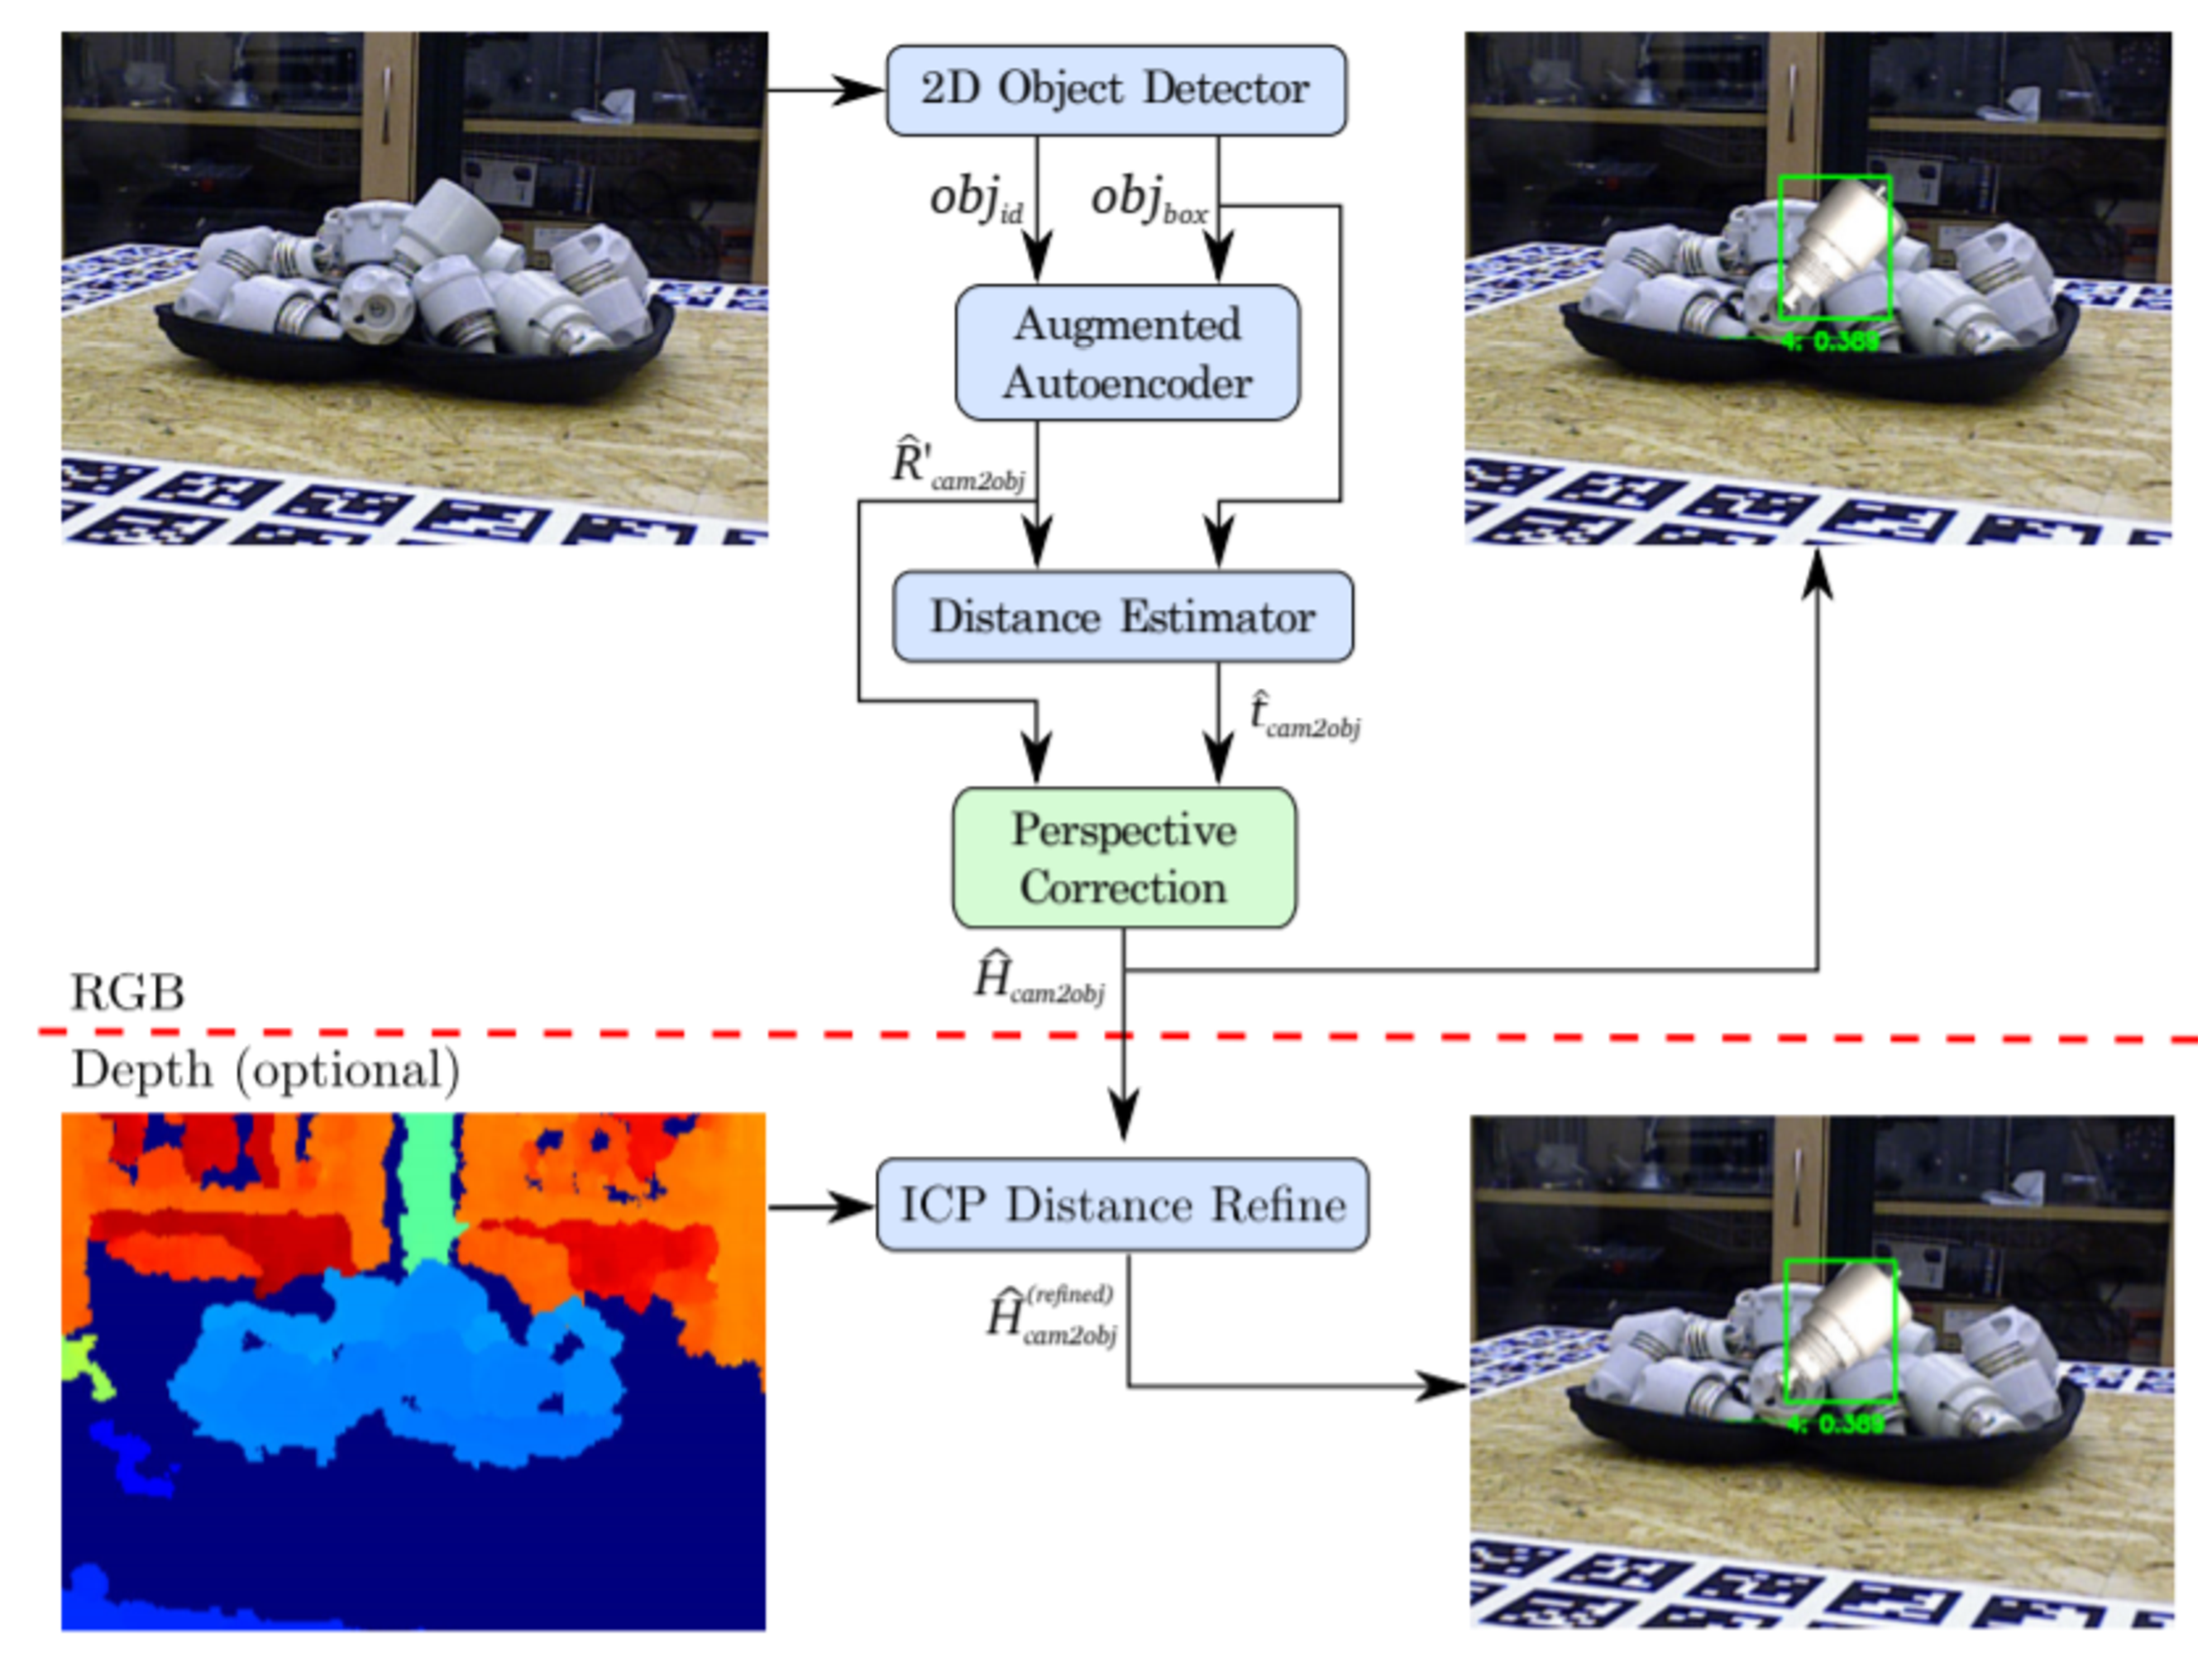
\includegraphics[width=100mm]{figure/eps/6次元推定.eps}
      \caption{6次元物体検出.}
      \label{fig:2d_pose_estimation}
      \end{center}
      \end{figure}



入力となるRGB画像に対してSSD\cite{SSD}を用いて対象物体のID,座標位置,Bounding Boxを検出する.
その後,検出されたBounding Box領域から物体の姿勢情報をAugumented Autoencoderにより取得し,推定を行う.
 


\subsection{Augumented Autoencoder}
AAEの基礎となるのがAutoencoder\cite{AE}である,オートエンコーダーは訓練データのみを使用する教師なし学習の一つである.入力データ$x_i$をエンコーダー$\phi$に入力し,デコーダ$\psi$から得られる出力$x’_i$との損失関数式(\ref{eq:polynomial2})を計算し学習を行い,データを表現する潜在変数zを獲得するためのニューラルネットワークである.潜在変数は式(\ref{eq:polynomial1})によって求められる.

\begin{eqnarray}
\label{eq:polynomial2}
l_2=  \sum_{i}\parallel{ x_i - x'_i} \parallel_2
\end{eqnarray}

\begin{eqnarray}
\label{eq:polynomial1}
( x ^ {\prime})  = (\psi \times  \phi )( x ) = \psi (z)
\end{eqnarray}



AAEでは,オートエンコーダーを発展させたノイズ除去を行い潜在変数を取得するDenoising Autoencoder\cite{DAE}が応用されている.
エンコーダーに訓練データの一部にノイズを加えた画像を入力し,ノイズなしの画像を出力できるよう,
ノイズのない訓練データとの損失関数を学習させることで,
ノイズによらない本質的な潜在表現を得ることができる方法である.

また,Domain Randomization\cite{Dm}という手法も取り入れられている.
この手法の目的は,評価時にモデルが実世界のデータに一般化できるよう,
環境ノイズを加えた3Dモデルをランダムに作成し学習を行う.
これにより物体と背景の対称性を明確にして,評価時に現実世界での推定も可能になる.

上記のDenoising AutoencoderとDomain Randomizationの手法を取り入れ応用したオートエンコーダーがAAEである.
AAEの学習を図\ref{AAEgakusyu}に示す.図\ref{AAEgakusyu}(a)の訓練データxに背景や光,遮蔽物などの環境ノイズ$f_augm$を追加した図\ref{AAEgakusyu}(b)の画像x''を入力し,環境ノイズなしの図\ref{AAEgakusyu}(c)の画像x'を出力するように
xとx"損失関数を計算し学習を行う.データを表現する潜在変数を式(\ref{eq:polynomial3})によって獲得する手法である.

      \begin{figure}[htbp]
      \begin{center}
      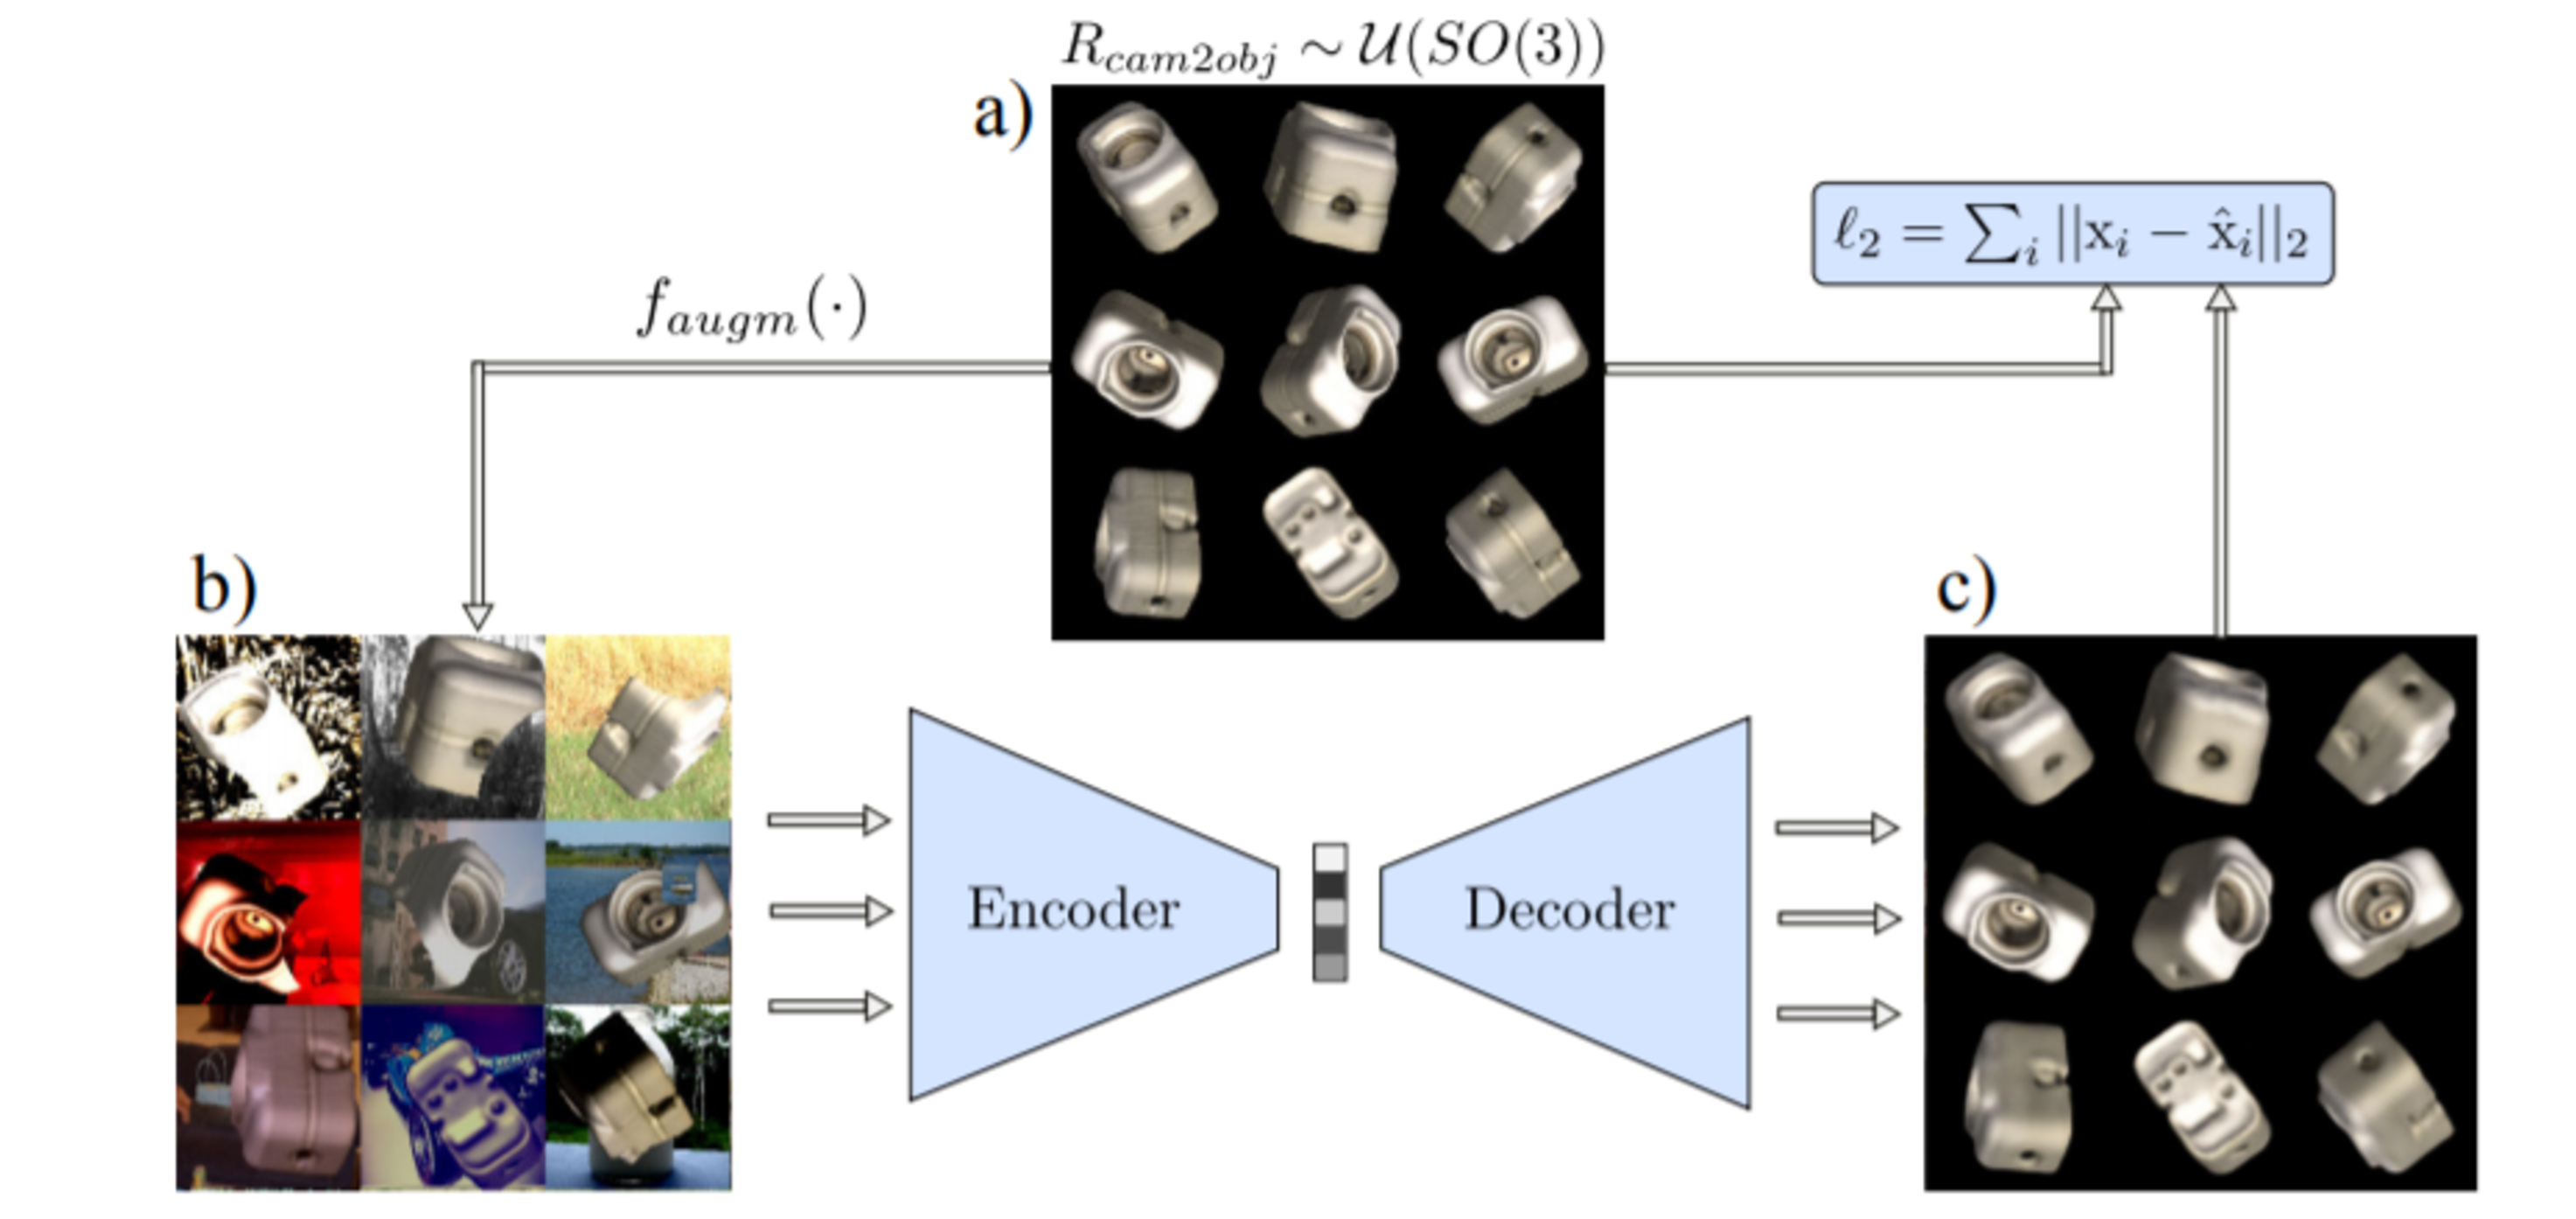
\includegraphics[width=110mm]{figure/eps/AAEの学習.eps}
      \caption{AAEの学習\cite{AAE}.}
      \label{AAEgakusyu}
      \end{center}
      \end{figure}

\begin{eqnarray}
\label{eq:polynomial3}
x ' = (\psi \times  \phi \times f_{augm} )( x ) = (\psi \times \phi) (x'') = \psi (z)
\end{eqnarray}


AAEのネットワークを図\ref{netwa}に示す.入力出力はチャンネル数3の画像サイズ128$\times$128のカラー画像を使用する.

      \begin{figure}[htbp]
      \begin{center}
      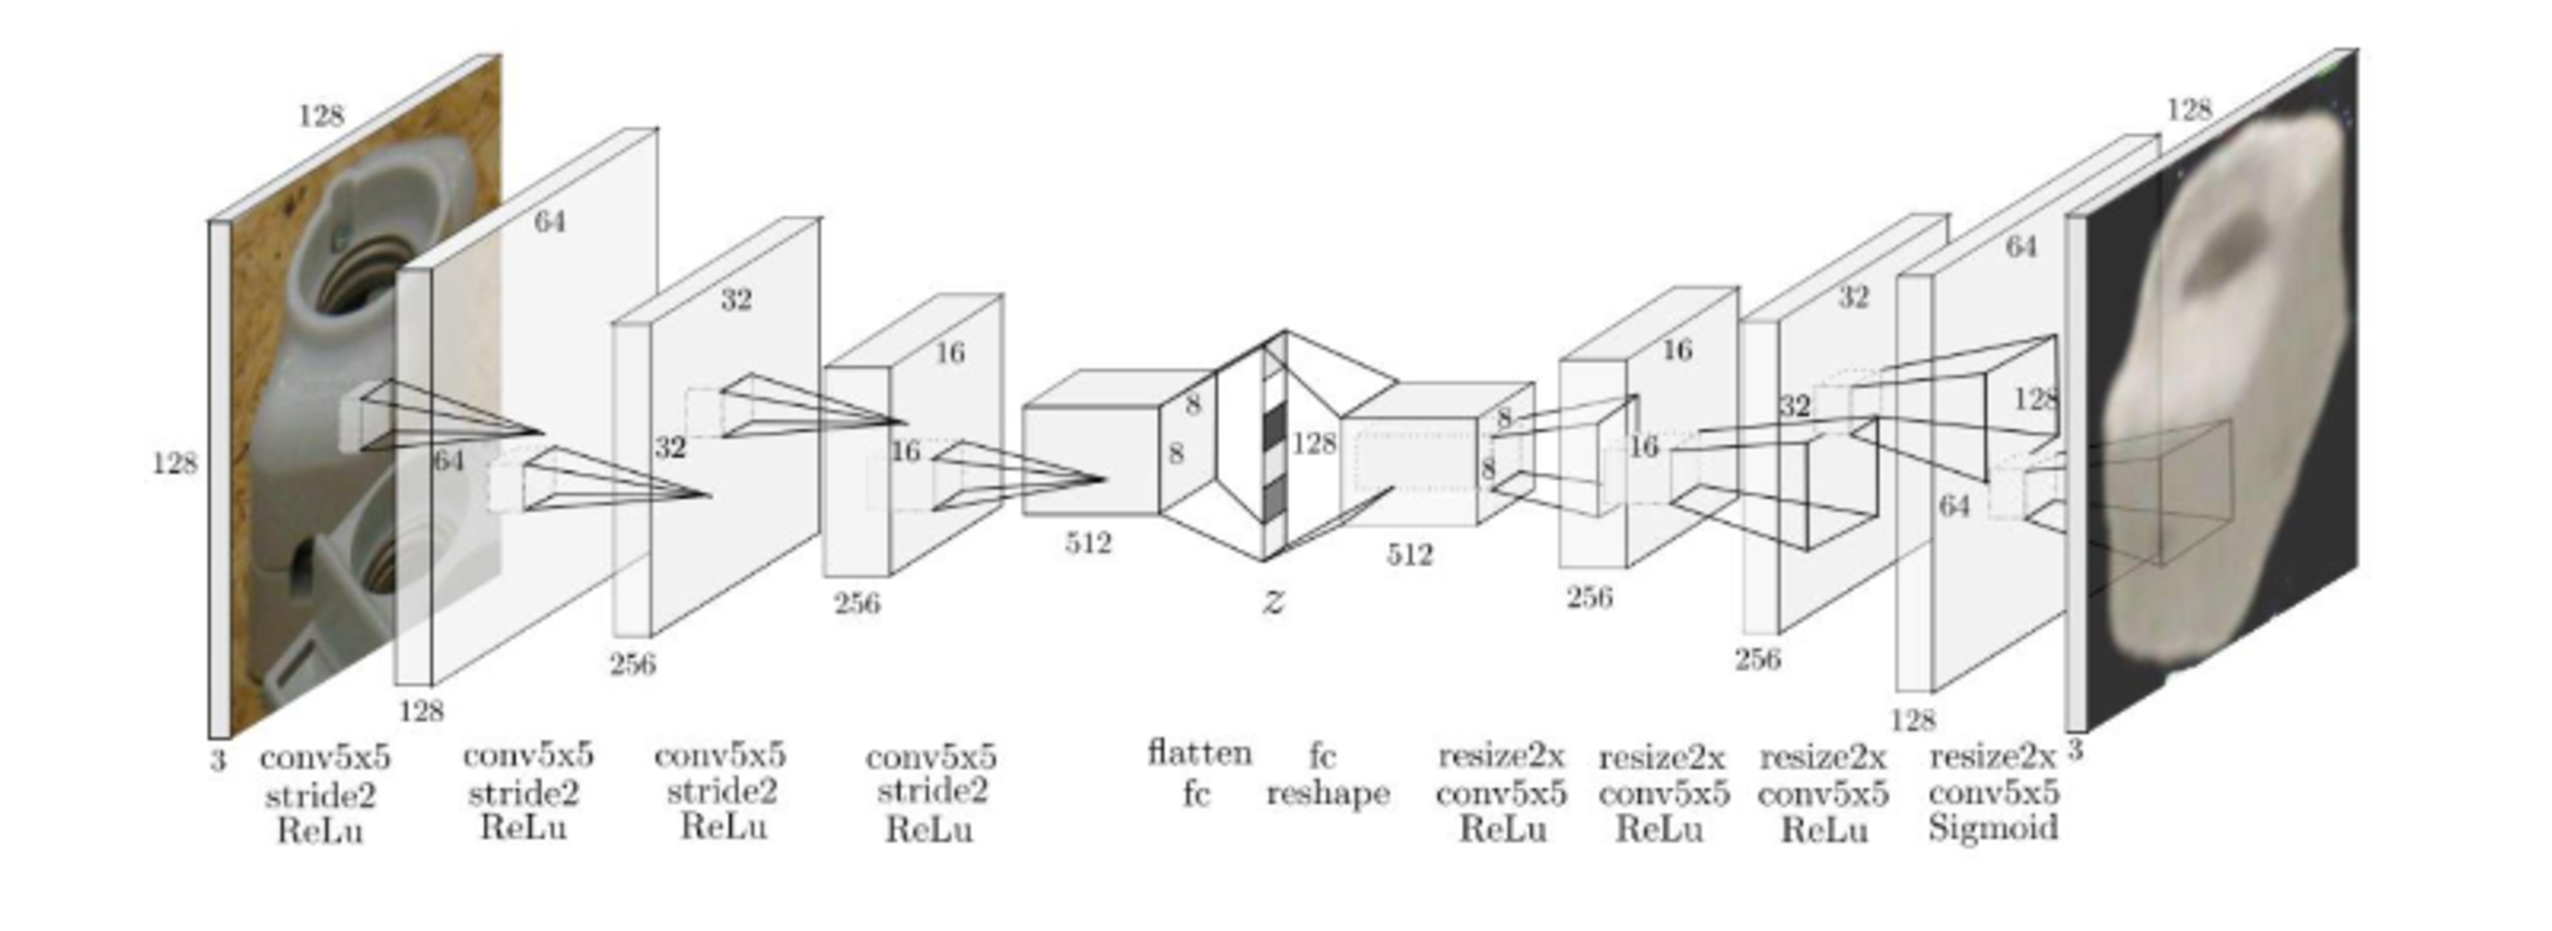
\includegraphics[width=120mm]{figure/eps/ネットワーク.eps}
      \caption{AAEのネットワーク\cite{AAE}.}
      \label{netwa}
      \end{center}
      \end{figure}





\subsection{AAEを用いた姿勢推定}


AAEによって求められる潜在変数を元に姿勢推定を行う.
推定対象となる物体の3Dモデルを作成し,3Dモデル物体を回転させ92232個の姿勢をAAEにかけ潜在変数を生成し92232個分の姿勢情報を持つ潜在変数を記録していく.
記録されている姿勢情報が既知となっている潜在変数$ z_i $と推定したい画像から新たに得た潜在変数$z_{test}$のコサイン類似度を式(\ref{cos})用いて比較し
最も近い潜在変数を持つ姿勢情報を推定姿勢として決定する.

\begin{eqnarray}
\label{cos}
cos_i = \frac {z_i \times z_{test}}{|z_i||z_{test}|}
\end{eqnarray}


%----------------------------------------------

%----------------------------------------------
\chapter*{おわりに}
\label{chap:10}
\markboth{おわりに}{}
\addcontentsline{toc}{chapter}{おわりに}
本研究では,機械学習を用いたARマーカの位置姿勢推定を提案し,評価実験より,
機械学習によって変形したARマーカの姿勢を推定できることを確認した.
今後は復元精度と姿勢推定の精度の向上を考えた学習方法と,現実空間においてリアルタイム
での復元及び姿勢推定する方法の研究を行う予定である.
%----------------------------------------------



%%%%%%%%%%%%%%%%%%%%%%%%%%%%%%%%%%%%%%%%%%%%%%%%%%%%%%%%%%%%%%%%
\chapter*{謝 辞}
\markboth{謝 辞}{}
\addcontentsline{toc}{chapter}{謝  辞}
本研究を行うにあたり,終始懇切なるご指導を頂きました中部大学工学部 XXXXX教授に謹んで感謝します.
次に,本論文の作成にあたり,有意義なご助言,ご指導頂いた
XXXX大学工学部 XXXXX教授,
XXXX大学大学院工学研究科情報工学専攻 XXXX氏に心から厚く御礼申し上げます.
最後に,本研究において,助言や相談,実験データ取得に協力して頂いたXXXX研究室の皆様に感謝致します.
%%%%%%%%%%%%%%%%%%%%%%%%%%%%%%%%%%%%%%%%%%%%%%%%%%%%%%%%%%%%%%%%
\cleardoublepage
\markboth{参考文献}{}     %% BibTeX を使う
%\bibliographystyle{jalpha}
%\newcommand{\noop}[1]{}
%\bibliographystyle{jabbrv}
\bibliographystyle{junsrt}
\bibliography{reference}
%\nocite{*}
%\bibliography{./ref}


%%%%%%%%%%%%%%%%%%%%%%%%%%%%%%%%%%%%%%%%%%%%%%%%%%%%%%%%%%%%%%%%
%%% 必要に応じて付録を作る
%%%%%%%%%%%%%%%%%%%%%%%%%%%%%%%%%%%%%%%%%%%%%%%%%%%%%%%%%%%%%%%%
% \chapter*{付  録}
% \markboth{付  録}{}
% \addcontentsline{toc}{chapter}{付  録}

%%%%%%%%%%%%%%%%%%%%%%%%%%%%%%%%%%%%%%%%%%%%%%%%%%%%%%%%%%%%%%%%

%%%%%%%%%%%%%%%%%%%%%%%%%%%%%%%%%%%%%%%%%%%%%%%%%%%%%%%%%%%%%%%%
%%% 必要に応じて論文目録を作る
%%%%%%%%%%%%%%%%%%%%%%%%%%%%%%%%%%%%%%%%%%%%%%%%%%%%%%%%%%%%%%%%



%%%%%%%%%%%%%%%%%%%%%%%%%%%%%%%%%%%%%%%%%%%%%%%%%%%%%%%%%%%%%%%%

\backmatter         %%% 奥付
\thispagestyle{empty}
\vspace*{18cm}
\begin{flushright}
\begin{tabular}{r}
\Hline
%\large
{論文題目}\\
(中部大学工学部ロボット理工学科)\\
ER00000\\
中部 太郎\\
20XX年 X月X日\\ %(卒業研究発表会の日時とする)

\Hline
\end{tabular}
\end{flushright}
\end{document}